% Options for packages loaded elsewhere
\PassOptionsToPackage{unicode}{hyperref}
\PassOptionsToPackage{hyphens}{url}
\documentclass[
  ignorenonframetext,
]{beamer}
\newif\ifbibliography
\usepackage{pgfpages}
\setbeamertemplate{caption}[numbered]
\setbeamertemplate{caption label separator}{: }
\setbeamercolor{caption name}{fg=normal text.fg}
\beamertemplatenavigationsymbolsempty
% remove section numbering
\setbeamertemplate{part page}{
  \centering
  \begin{beamercolorbox}[sep=16pt,center]{part title}
    \usebeamerfont{part title}\insertpart\par
  \end{beamercolorbox}
}
\setbeamertemplate{section page}{
  \centering
  \begin{beamercolorbox}[sep=12pt,center]{section title}
    \usebeamerfont{section title}\insertsection\par
  \end{beamercolorbox}
}
\setbeamertemplate{subsection page}{
  \centering
  \begin{beamercolorbox}[sep=8pt,center]{subsection title}
    \usebeamerfont{subsection title}\insertsubsection\par
  \end{beamercolorbox}
}
% Prevent slide breaks in the middle of a paragraph
\widowpenalties 1 10000
\raggedbottom
\AtBeginPart{
  \frame{\partpage}
}
\AtBeginSection{
  \ifbibliography
  \else
    \frame{\sectionpage}
  \fi
}
\AtBeginSubsection{
  \frame{\subsectionpage}
}
\usepackage{iftex}
\ifPDFTeX
  \usepackage[T1]{fontenc}
  \usepackage[utf8]{inputenc}
  \usepackage{textcomp} % provide euro and other symbols
\else % if luatex or xetex
  \usepackage{unicode-math} % this also loads fontspec
  \defaultfontfeatures{Scale=MatchLowercase}
  \defaultfontfeatures[\rmfamily]{Ligatures=TeX,Scale=1}
\fi
\usepackage{lmodern}
\ifPDFTeX\else
  % xetex/luatex font selection
\fi
% Use upquote if available, for straight quotes in verbatim environments
\IfFileExists{upquote.sty}{\usepackage{upquote}}{}
\IfFileExists{microtype.sty}{% use microtype if available
  \usepackage[]{microtype}
  \UseMicrotypeSet[protrusion]{basicmath} % disable protrusion for tt fonts
}{}
\makeatletter
\@ifundefined{KOMAClassName}{% if non-KOMA class
  \IfFileExists{parskip.sty}{%
    \usepackage{parskip}
  }{% else
    \setlength{\parindent}{0pt}
    \setlength{\parskip}{6pt plus 2pt minus 1pt}}
}{% if KOMA class
  \KOMAoptions{parskip=half}}
\makeatother
\usepackage{longtable,booktabs,array}
\newcounter{none} % for unnumbered tables
\usepackage{calc} % for calculating minipage widths
\usepackage{caption}
% Make caption package work with longtable
\makeatletter
\def\fnum@table{\tablename~\thetable}
\makeatother
\usepackage{graphicx}
\makeatletter
\newsavebox\pandoc@box
\newcommand*\pandocbounded[1]{% scales image to fit in text height/width
  \sbox\pandoc@box{#1}%
  \Gscale@div\@tempa{\textheight}{\dimexpr\ht\pandoc@box+\dp\pandoc@box\relax}%
  \Gscale@div\@tempb{\linewidth}{\wd\pandoc@box}%
  \ifdim\@tempb\p@<\@tempa\p@\let\@tempa\@tempb\fi% select the smaller of both
  \ifdim\@tempa\p@<\p@\scalebox{\@tempa}{\usebox\pandoc@box}%
  \else\usebox{\pandoc@box}%
  \fi%
}
% Set default figure placement to htbp
\def\fps@figure{htbp}
\makeatother
\setlength{\emergencystretch}{3em} % prevent overfull lines
\providecommand{\tightlist}{%
  \setlength{\itemsep}{0pt}\setlength{\parskip}{0pt}}
\usepackage{bookmark}
\IfFileExists{xurl.sty}{\usepackage{xurl}}{} % add URL line breaks if available
\urlstyle{same}
\hypersetup{
  hidelinks,
  pdfcreator={LaTeX via pandoc}}

\author{\texorpdfstring{}{}}
\date{}

\begin{document}

\begin{frame}[fragile]{Results}
\protect\phantomsection\label{results}
All numbers below come from \texttt{output/data/proximity\_summary.json}
after running \texttt{scripts/proximity\_monte\_carlo.py} with
\texttt{q\_max=120}, \texttt{n\_uniform=4000},
\texttt{n\_quadratic=2000}, \texttt{n\_beta=1000} (Jeffreys prior on
\((0,1)\)), seed \texttt{20260322} (see
\texttt{manuscript/config.yaml}). The same JSON carries
\texttt{reference\_summary} for the pooled sample. Independent checks of
the \(\delta_Q\) implementation appear in
\texttt{output/data/lattice\_crosscheck.json} from
\texttt{02\_lattice\_crosscheck.py}.

\begin{block}{Empirical percentiles of \(\delta_{120}(x^\star)\)}
\protect\phantomsection\label{empirical-percentiles-of-delta_120xstar}
{\def\LTcaptype{none} % do not increment counter
\begin{longtable}[]{@{}
  >{\raggedright\arraybackslash}p{(\linewidth - 4\tabcolsep) * \real{0.1389}}
  >{\raggedright\arraybackslash}p{(\linewidth - 4\tabcolsep) * \real{0.3472}}
  >{\raggedright\arraybackslash}p{(\linewidth - 4\tabcolsep) * \real{0.5139}}@{}}
\toprule\noalign{}
\begin{minipage}[b]{\linewidth}\raggedright
Constant
\end{minipage} & \begin{minipage}[b]{\linewidth}\raggedright
\(\delta_{120}(x^\star)\)
\end{minipage} & \begin{minipage}[b]{\linewidth}\raggedright
empirical rank in pooled reference
\end{minipage} \\
\midrule\noalign{}
\endhead
\texttt{one\_sixth} (rational) & \(0\) & \(0\) \\
\texttt{pi} & \(2.67\times 10^{-7}\) & \(0.00171\) \\
\texttt{e} & \(2.80\times 10^{-5}\) & \(0.192\) \\
\texttt{ln2} & \(3.46\times 10^{-5}\) & \(0.279\) \\
\texttt{golden\_ratio} & \(5.65\times 10^{-5}\) & \(0.498\) \\
\texttt{sqrt2} & \(7.21\times 10^{-5}\) & \(0.574\) \\
\texttt{sqrt3} & \(9.20\times 10^{-5}\) & \(0.718\) \\
\bottomrule\noalign{}
\end{longtable}
}

The rational control hits zero distance as soon as \(Q\) is a multiple
of the true denominator, confirming the end-to-end path from
\texttt{rational\_distance.py} through aggregation. \(\pi\) occupies an
extreme left tail at this \(Q\)---consistent with the existence of
exceptionally accurate low-height rationals (e.g., \(355/113\)) that
remain admissible when \(Q=120\).
\end{block}

\begin{block}{Histogram}
\protect\phantomsection\label{histogram}
Figure \ref{fig:proximity_hist} shows the base-10 logarithm of
\(\delta_{120}(U)\) for uniform draws, with vertical markers for
\(\pi\), \(\sqrt{2}\), \(\varphi\), and \(\ln 2\).

\begin{figure}
\centering
\pandocbounded{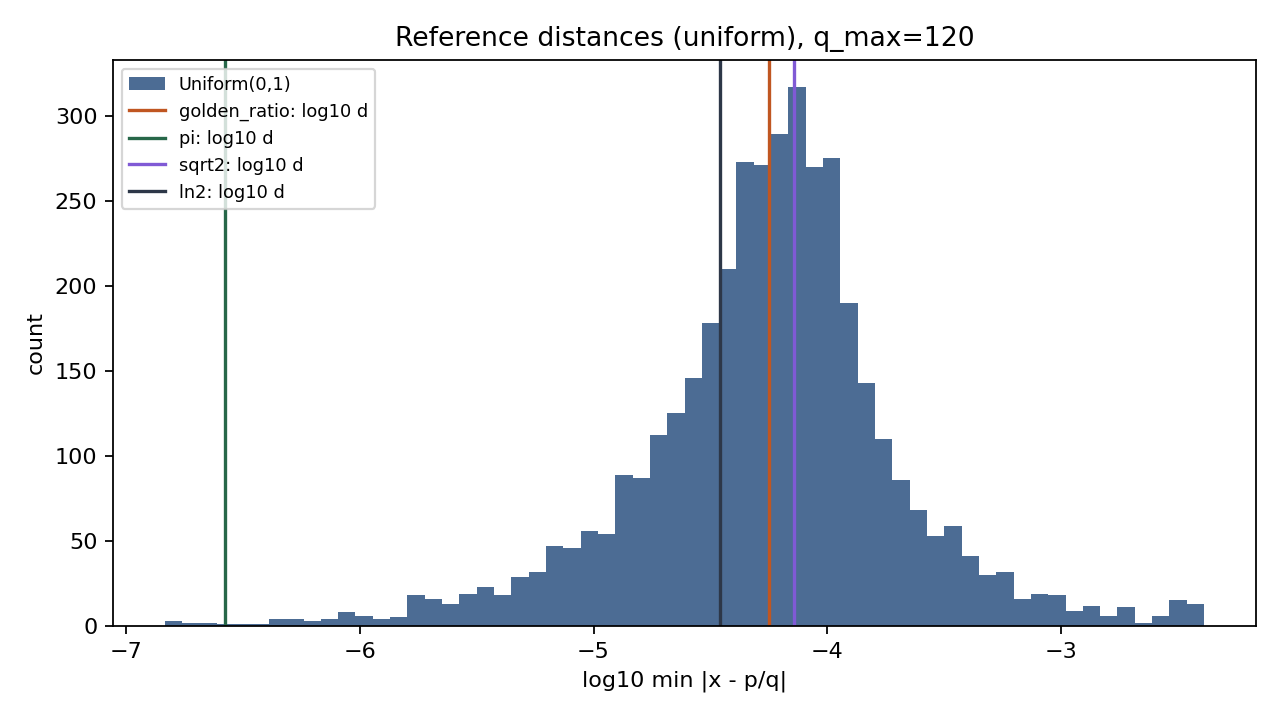
\includegraphics[keepaspectratio,alt={Empirical distribution of \textbackslash log\_\{10\} \textbackslash delta\_\{120\} for uniform references with marker lines for selected constants.}]{../figures/proximity_histogram.png}}
\caption{Empirical distribution of \(\log_{10} \delta_{120}\) for
uniform references with marker lines for selected
constants.}\label{fig:proximity_hist}
\end{figure}

The pooled reference (not plotted) adds quadratic-mod-\(1\) samples;
table ranks use that pooled empirical CDF.
\end{block}
\end{frame}

\end{document}
